\section{Terraform}

\subsection{Basics}
Infrastructure reqirements for deploying applications include VMs, security, network access, firewall rules, 
availability and maintainability.

Terraform is responsible for deploying and maintaining infrastructure. It supports infrastructure providers such as AWS,
 Microsoft Azure, Google Cloud and many more via provider plugins.

These plugins convert the terraform calls into something that can communicate with the client SDK of the cloud provider. 

Terraform commands are written in Hashicorp Configuration Language HCL which
\begin{itemize}
    \item is simple, easy to learn
    \item has in-built type system
    \item supports for-loops, dynamic blocks, contitionals and string interpolation
\end{itemize}

The terraform language consists of blocks, arguments (assigning values to a name) and expressions.

\begin{figure}[h]
    \centering
    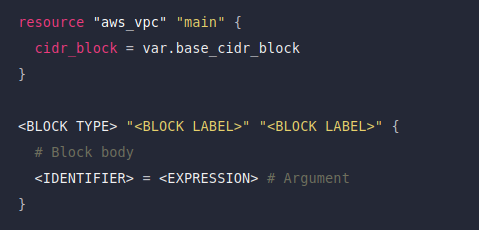
\includegraphics[width=\textwidth]{terraform-language}
\end{figure}

A Terraform configuration is a complete document in the Terraform language that tells Terraform
 how to manage a given collection of infrastructure. 
A configuration can consist of multiple files and directories.

\subsection{Components}
\textbf{version.tf} -- describes which terraform version and which providers are required 

\noindent
\textbf{provider.tf} -- contains access keys, etc.

\noindent
\textbf{main.tf} -- contains actual infrastructure descriptions

\vspace{3mm}
\noindent
\textbf{terraform init} -- initializes working directory with specified provider selections, etc.

\noindent
\textbf{terraform plan} -- calculate the changes based on declarations and state, display what would be executed

\noindent
\textbf{terraform apply} -- run the deployment, create, update or delete resources as needed

\noindent
\textbf{terraform destroy} -- remove all resources defined in terraform configuration files

\vspace{3mm}
\noindent
\textbf{.tfstate} -- current state information. is used for terraform plan command.

\subsection{Resource referencing}
$<$ResourceType$>$.$<$Name$>$ represents a managed resource of the given type and name.

VAR.$<$Name$>$ is the value of an input variable oof the given name.

\subsection{Outputs}

\subsection{Data}

\subsection{State file sharing}
The state file \emph{terraform.tfstate} kept for every environment is best stored in a central location when working in a team.
Remote storage providers enable locking of the state file for every operation, in case several users apply modifications 
at the same time.

The refresh operation synchronizes the state file with the actual status of the managed infrastructure and maps object IDs to
the resource instances defined inside terraform configuration. 

\subsection{Modules for Code Reuse}
Modules are containers for multiple resources that are used together. 
A module consists of a collection of \emph{.tf} and / or \emph{.tf.json} files kept together in a directory.
 The root module is usually the main folder of the terraform resources. 